\chapter{Methodology}
\label{chap:methodology}

\lettrine[lines=3, findent=3pt, nindent=0pt]{C}{hapter} 3 deals with software and methodologies used for building the \gls{ids}. Starting with the concept behind the code, will then be discussed the scripts used, the pre-processing done to the chosen dataset, along with some statistics about the latter and the algorithms adopted in the \gls{ml} model training. In the final section will also be provided a \gls{poc} to demonstrate the functioning of the final product. The workflow has revolved around Git as \gls{vcs}\footnote{See appendix \ref{app:repository}}.

%----------------------------------------------------
% CONCEPT
%----------------------------------------------------

\section{Concept}
\label{sec:concept}

In this section will be explained the more abstract and high-level idea, on which the \gls{ids} was built. The concept is summarized by the following figure:

\begin{figure}[h!]
    \centering
    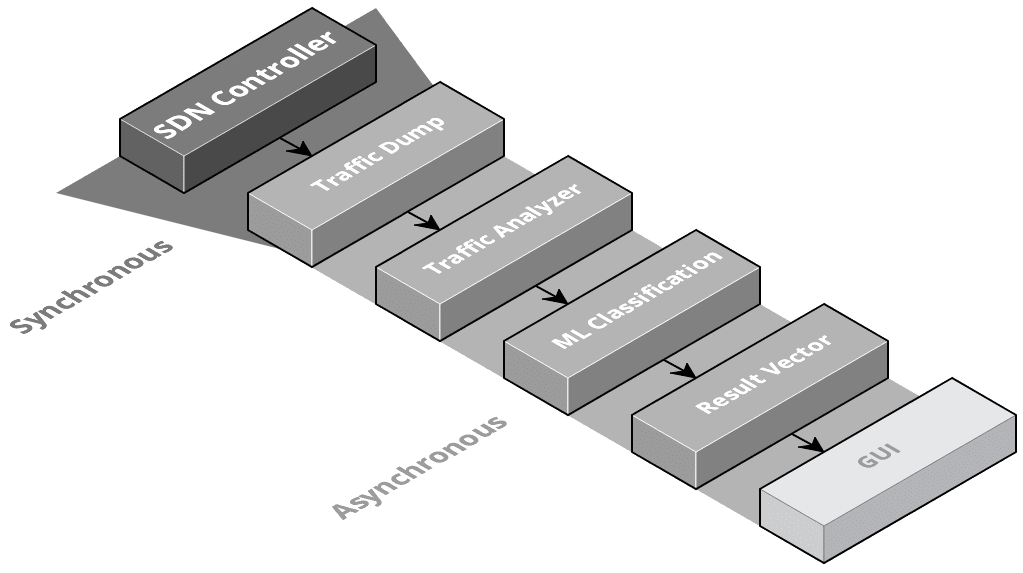
\includegraphics[scale=0.32]{assets/figures/chapter3/concept-components.png}
    \caption{Project's flowchart: from raw traffic to classified vector}
    \label{fig:concept-components}
\end{figure}

\noindent The system can be used in both, \textit{synchronous} or \textit{asynchronous} mode. Proceeding top-down, the \textit{SDN Controller} serves the purpose of orchestrating the duplication of network traffic\footnote{See section \ref{subsubsec:traffic-duplication}} in order to create a \gls{pcap} file (so called \textit{traffic dump}) every 30 seconds. The latter will be than passed to the \textit{Analyzer}, which has the task of converting the traffic dump into a vector and pass it to the \gls{ml} model, in order to perform classification. The Analyzer can also get user uploaded files as input, and this allows the asynchronous operation. The \textit{\gls{ml} Classification} block consists of passing the previously mentioned vector to the trained \gls{rf} model and appending periodically the results to a \glsxtrshort{csv} file. In the final step, the \textit{Result Vector} can be visualized using the web \gls{gui}.

%----------------------------------------------------
% MODEL TRAINING
%----------------------------------------------------

\section{\gls{ml} Model Training}
\label{sec:model-training}

This is the first stage of the implementation. For this purpose was used a \textit{Jupyter Notebook} to pre-process and visualize the raw data and then to train the \gls{ml} model. For reference, all the operations described were done using a MacBook Pro with 8 GB of RAM and an iMac with 16 GB of RAM, both running macOS 11.4 (Big Sur). The datasets used, as discussed in \ref{subsec:datasets-for-evaluation}, are NSL-KDD and CICIDS2017. The former was only used to become familiar with \gls{ml} and Jupyter Notebooks in general, the latter was the one strictly useful to the project.

%----------------------------------------------------
% PRE-PROCESSING
%----------------------------------------------------

\subsection{Pre-Processing}
\label{subsec:pre-processing}

After the dataset choice, \textit{pre-processing} is very important in order to get consistent results regarding the training of the \gls{ml} model, and so the accuracy of the \gls{ids}. It is important to remove redundant or null records and unimportant features. The dataset used contains plenty records so \texttt{NaN}, \texttt{Null} and \texttt{Inf} values were dropped to clean the data the model will work with. Also columns containing non numerical values were dropped (\texttt{Flow\_ID}, \texttt{Source\_IP}, \texttt{Destination\_IP}, \texttt{Timestamp}), except the one containing the traffic category (\texttt{Label}). \\ In order to visualize and comprehend what is going on, Python's \textit{Pandas Library} \cite{PandasLibrary} was the choice. Printing the dataset's value counts helps to understand the ratio between normal traffic and malicious one. 

\begin{table}[h]
    \centering
    \begin{tabular}{l|l}
        \toprule 
        Traffic Label & Entries \\
        \midrule
        \rowcolor{black!10} Benign & 2,271,320 \\
        DoS Hulk & 230,124 \\
        \rowcolor{black!10} Port Scan & 158,804 \\
        DDoS & 128,025 \\
        \rowcolor{black!10} DoS GoldenEye & 10,293 \\
        FTP-Patator & 7,935 \\
        \rowcolor{black!10} SSH-Patator & 5,897 \\
        DoS Slowloris & 5,796 \\
        \rowcolor{black!10} DoS Slowhttptest & 5,499 \\
        Bot & 1,956 \\
        \rowcolor{black!10} Web Attack: Brute Force & 1,507 \\
        Web Attack: XSS & 652 \\
        \rowcolor{black!10} Infiltration & 36 \\
        Web Attack: SQL Injection & 21 \\
        \rowcolor{black!10} Heartbleed & 11 \\
        \bottomrule
    \end{tabular}
    \caption{CICIDS2017 (ungrouped) Value Counts}
    \label{tab:dataset-distribution}
\end{table}

\noindent From the above table comes clear that there are traffic categories with insufficient data to train the model, and have to be dropped (Infiltration, SQL Injection and Heartbleed). The remaining 12 labels were than grouped by relevance according to the table below, in order to generalize the categorization.

\begin{table}[h]
    \centering
    \begin{tabular}{l|l|l}
        \toprule 
        Group Name & Labels & Entries \\
        \midrule
        \rowcolor{black!10} Benign & Benign & 2,271,320 \\
        Dos & DoS Hulk, DoS GoldenEye, DoS Slowloris, DoS Slowhttptest &  251,712 \\
        \rowcolor{black!10}Probe & Port Scan & 158,804 \\
        DDoS & DDoS & 128,025 \\
        \rowcolor{black!10}Brute Force & FTP-Patator, SSH-Patator  & 13,832 \\
        Web Attack & Web Attack: Brute Force, Web Attack: XSS & 2,159 \\
        \rowcolor{black!10}Botnet & Bot & 1,956 \\
        \bottomrule
    \end{tabular}
    \caption{CICIDS2017 (grouped) Value Counts}
    \label{tab:grouped-dataset-distribution}
\end{table}

\noindent Another step of the pre-processing stage consisted in splitting the dataset. Being the latter explicitly unbalanced, since it consists in 5 days of traffic acquisition, each one dedicated to a specific attack type, it was performed a \textit{stratified split}, using Pandas' \texttt{train\_test\_split()}, which splits arrays or matrices into train and test subsets, maintaining the same ratio of classes across the subsets. As pointed out in \cite{Mozley2020}, a fundamental step in pre-processing is \textit{normalization}: since the scale of the feature value differs, to ensure that each one of them contribute the same amount to the classification, it is mandatory to bring them to the same range. In Python it is possible to do a \textit{min-max normalization} using \texttt{scikit-learn} library \cite{ScikitWebsite}. This kind of operation re-scales the dataset's features using the following equation:

\begin{equation}
    x\prime=\frac{x-\min\{x\}}{\max\{x\}-\min\{x\}}
\end{equation}
In which $x$ is the feature's original value.

%----------------------------------------------------
% FEATURES AND STATISTICS
%----------------------------------------------------

\subsection{Features and Statistics}
\label{subsec:features-statistics}

As pointed out in \ref{subsec:traffic-characterization}, given a dataset, some features are more relevant than others. In order to achieve an higher accuracy and generalization and saving time in the training stage, the right move was using only the most relevant features in such a fashion that if the feature value and the class label are independent, then the elder is not relevant in the classification process, therefore it has to be dropped. The library of choice was \texttt{scikit-learn} \cite{ScikitWebsite}, and in particular it's \texttt{SelectKBest} function: this was helpful for selecting the top 40 (in this particular case) most dependent features of the dataset, using the \textit{chi-squared} algorithm. The chart below represents a plot of the features score mentioned earlier: to be noticed is the dotted line, which represents the $99\%$ mark, meaning that all the features above are not so relevant for the purpose.

\begin{figure}[h!]
    \centering
    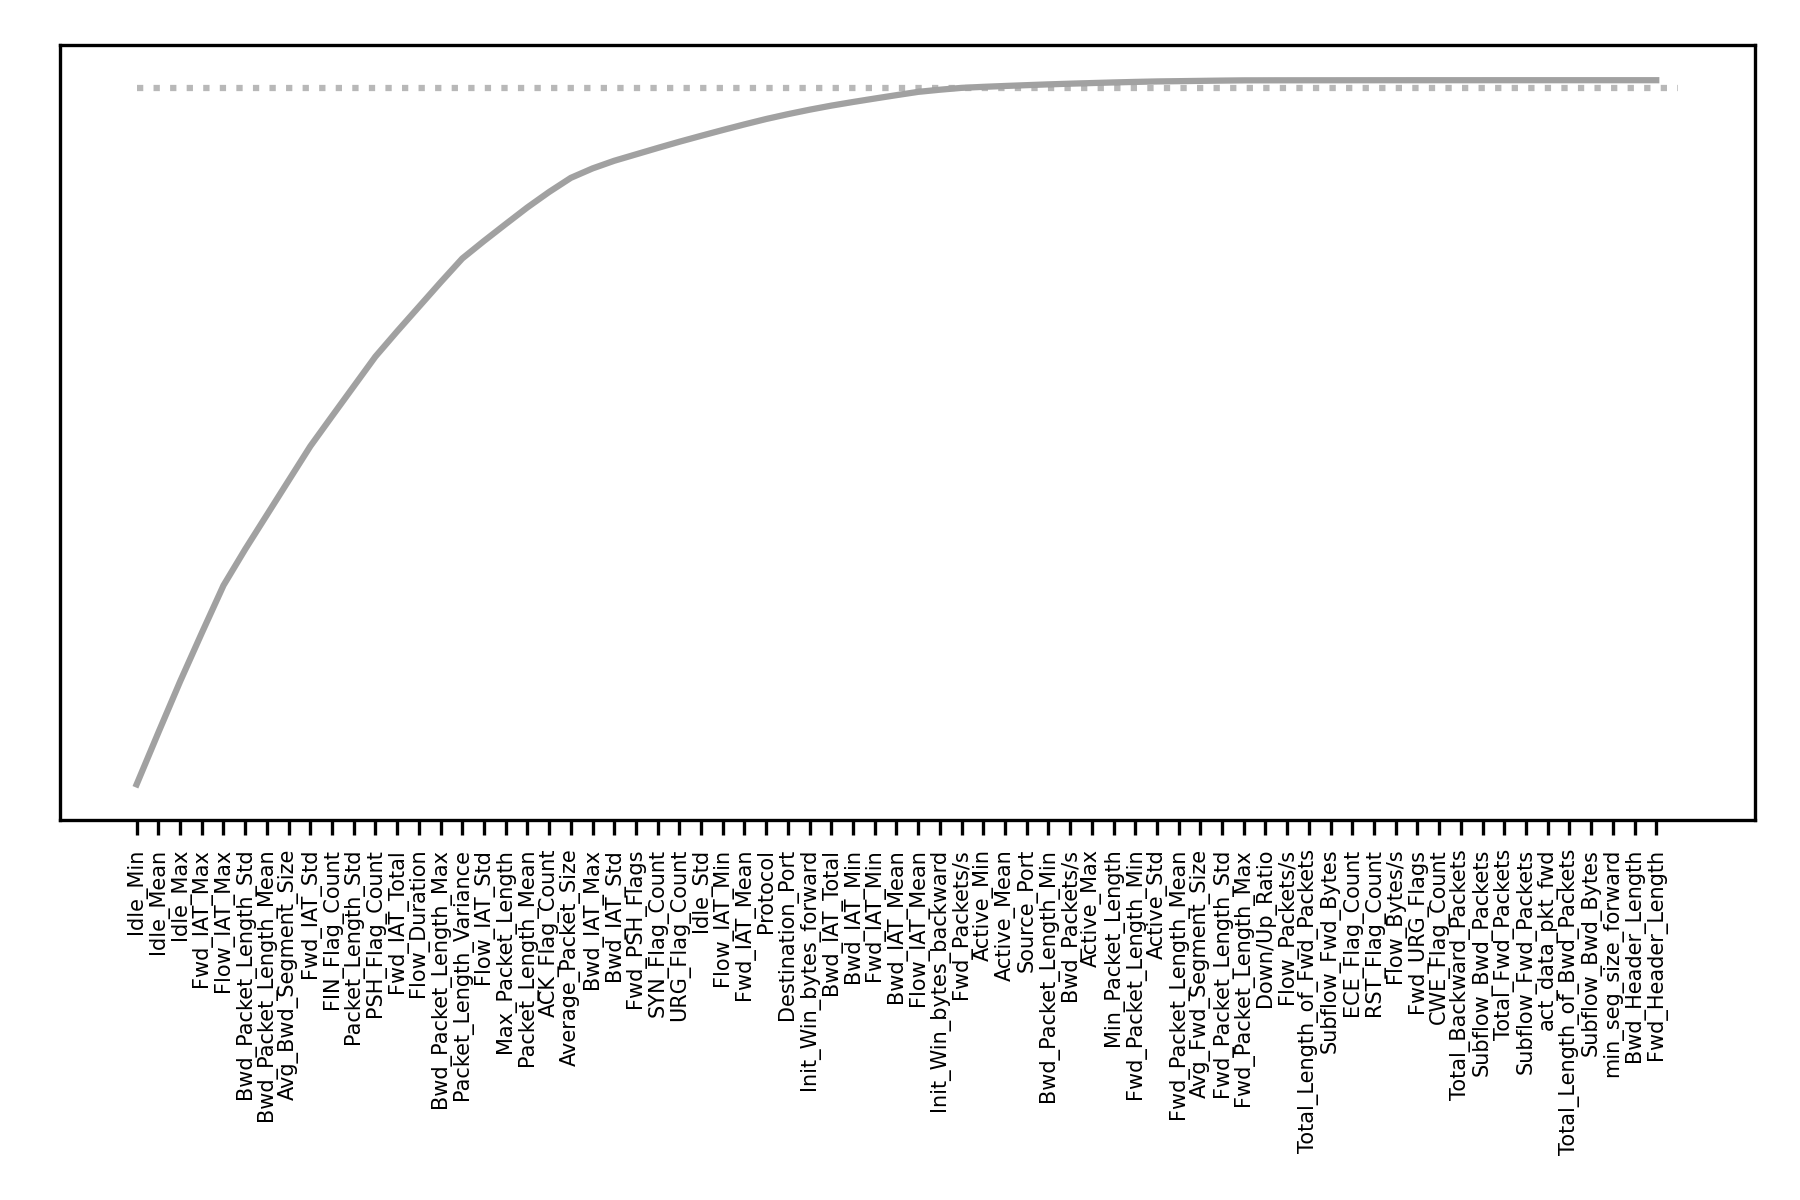
\includegraphics[scale=1]{assets/figures/chapter3/features99.png}
    \caption{CICIDS2017 Features Weight}
    \label{fig:features-weight}
\end{figure}

\noindent Table \ref{tab:features-weight} contains a list, along with the respective description of all the selected features, to summarize what was used in the training stage. For further data and statistics, see appendix \ref{app:net-features}.

\begin{table}[h]
    \centering
    \begin{tabular}{l|l}
        \toprule 
        Feature & Description \\
        \midrule
        \rowcolor{black!10} \texttt{Destination\_Port} & It follows a table  \\
        \texttt{Protocol} & DoS Hulk \\
        \rowcolor{black!10} \texttt{Flow\_Duration} & Port Scan \\
        \texttt{Bwd\_Packet\_Length\_Max} & Maximum size of packet in backward direction \\
        \rowcolor{black!10} \texttt{Bwd\_Packet\_Length\_Mean} & Mean size of packet in backward direction \\
        \texttt{Bwd\_Packet\_Length\_Std} & Standard deviation size of packet in backward direction \\
        \rowcolor{black!10} \texttt{Flow\_IAT\_Mean} & Mean time between two packets sent in the flow \\
        \texttt{Flow\_IAT\_Std} & Standard deviation time between two packets sent in the flow \\
        \rowcolor{black!10} \texttt{Flow\_IAT\_Max} & Maximum time between two packets sent in the flow \\
        \texttt{Flow\_IAT\_Min} & Minimum time between two packets sent in the flow \\
        \rowcolor{black!10} \texttt{Fwd\_IAT\_Total} & Total time between two packets sent in the forward direction \\
        \texttt{Fwd\_IAT\_Mean} & Mean time between two packets sent in the forward direction \\
        \rowcolor{black!10} \texttt{Fwd\_IAT\_Std} & Standard deviation time between two packets sent in the forward direction \\
        \texttt{Protocol} & DoS Hulk \\
        \rowcolor{black!10} \texttt{Flow\_Duration} & Port Scan \\
        \texttt{Bwd\_Packet\_Length\_Max} & DDoS \\
        \rowcolor{black!10} \texttt{Bwd\_Packet\_Length\_Mean} & FTP-Patator, SSH-Patator \\
        \texttt{Bwd\_Packet\_Length\_Std} & Web Attack: Brute Force, Web Attack: XSS \\
        \rowcolor{black!10} \texttt{Flow\_IAT\_Mean} & Bot \\
        \bottomrule
    \end{tabular}
    \caption{CICIDS2017 Features Weight and Description (most relevant to least relevant)}
    \label{tab:features-weight}
\end{table}

%\begin{figure}[h!]
%    \centering
%    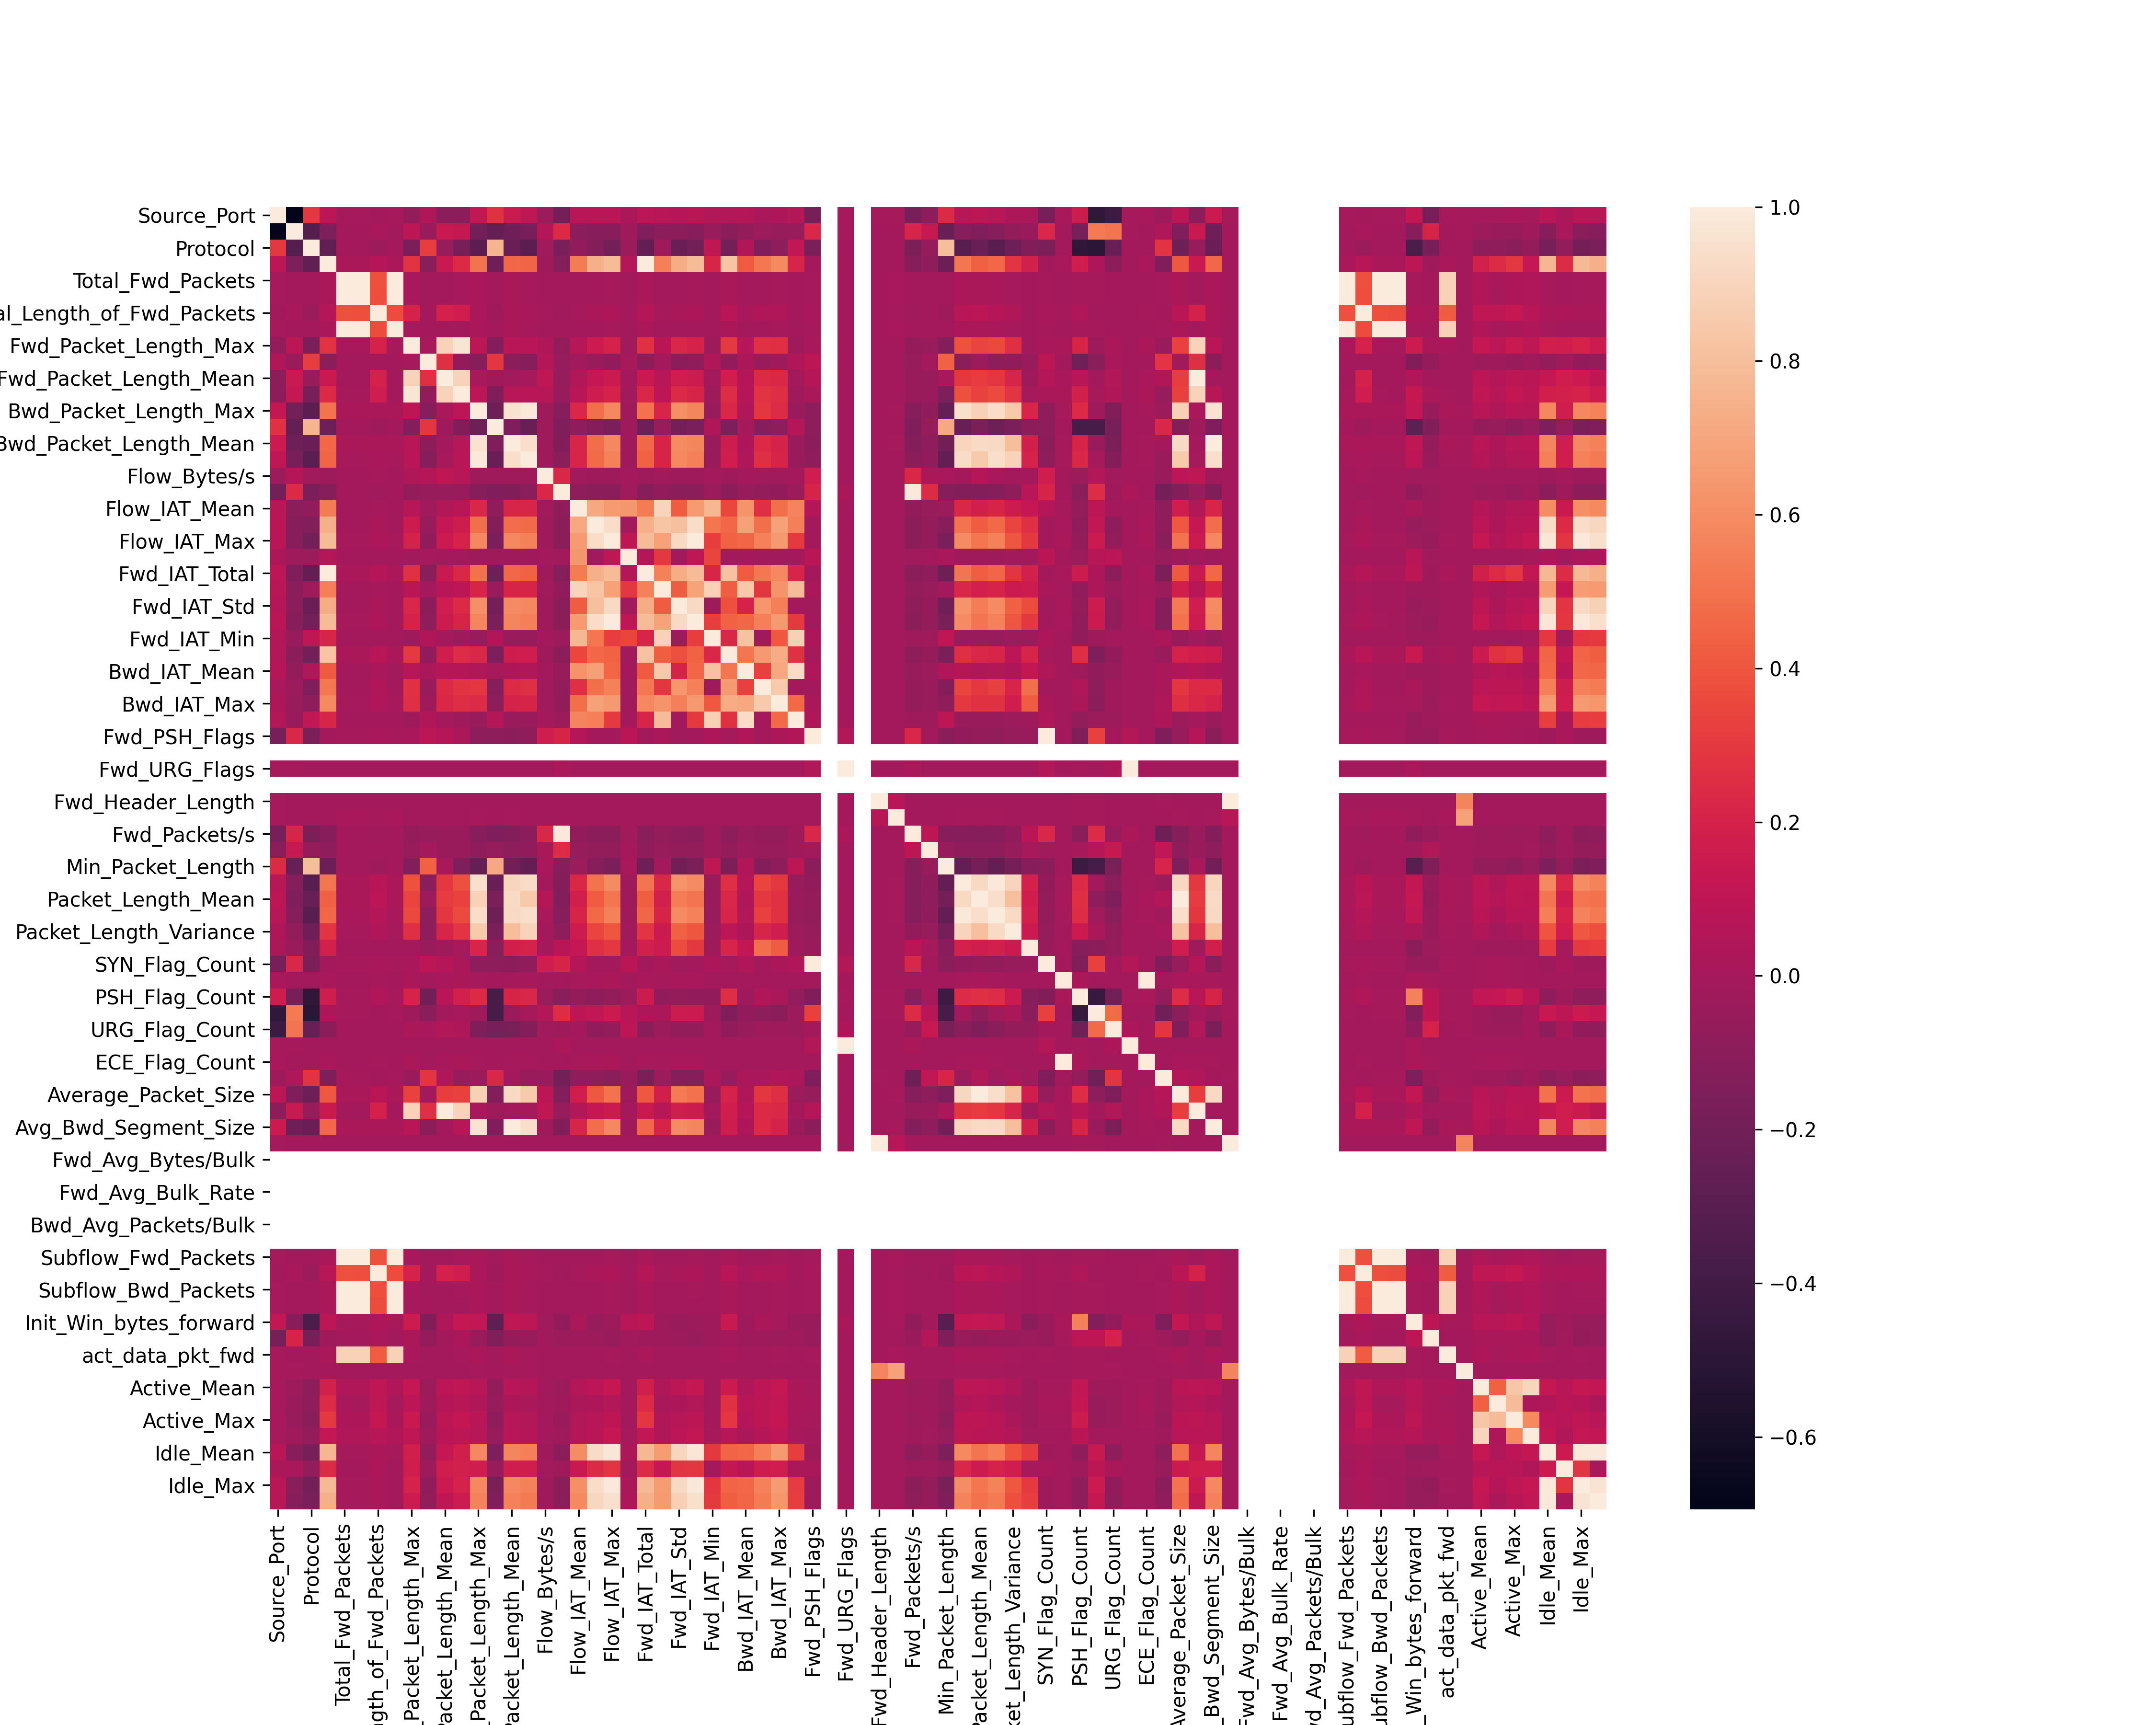
\includegraphics[scale=0.5]{assets/figures/chapter3/heatmap-all.png}
%    \caption{CICIDS2017 Feature Correlation Matrix (heatmap)}
%    \label{fig:feature-heatmap}
%\end{figure}

%----------------------------------------------------
% CLASSIFICATION
%----------------------------------------------------

\subsection{Classification}
\label{subsec:classification}

\textcolor{dimgray}{\lipsum[1]}

%----------------------------------------------------
% NETWORK MONITOR
%----------------------------------------------------

\section{Network Monitor}
\label{sec:monitor-implementation}

\textcolor{dimgray}{\lipsum[1]}

%----------------------------------------------------
% ML INTEGRATION
%----------------------------------------------------

\subsection{\gls{ml} Integration}
\label{subsec:ml-integration}

\textcolor{dimgray}{\lipsum[1]}

\begin{figure}
    \begin{code}[colback=white]{Monitor.py}
if packet.getFwdID() in current_flows.keys():
flow = current_flows[packet.getFwdID()]

# check for timeout
# for some reason they only do it if packet count > 1
if (packet.getTimestamp() - flow.getFlowStartTime()) > FlowTimeout:
    classify(flow.terminated())
    del current_flows[packet.getFwdID()]
    flow = Flow(packet)
    current_flows[packet.getFwdID()] = flow

# check for fin flag
elif packet.getFINFlag() or packet.getRSTFlag():
    flow.new(packet, 'fwd')
    classify(flow.terminated())
    del current_flows[packet.getFwdID()]
    del flow
\end{code}
\end{figure}

\textcolor{dimgray}{\lipsum[1]}

%----------------------------------------------------
% MONITORING PIPELINE
%----------------------------------------------------

\subsection{Monitoring Pipeline}
\label{subsec:monitoring-pipeline}

\textcolor{dimgray}{\lipsum[1]}

%----------------------------------------------------
% POC
%----------------------------------------------------

\section{Proof of Concept}
\label{sec:poc}

\textcolor{dimgray}{\lipsum[1-10]}

%----------------------------------------------------
% TRAFFIC ACQUISITION
%----------------------------------------------------

\subsection{Traffic Acquisition}
\label{subsec:traffic-acquisition}

\textcolor{dimgray}{\lipsum}

%----------------------------------------------------
% TOPOLOGY
%----------------------------------------------------

\subsection{Topology}
\label{subsec:topology}

\textcolor{dimgray}{\lipsum}
